\chapter{Automatic generation of labels for topics' bags of words}
\doublespacing
\label{chap:label}
\minitoc



\section{Introduction: find labels to represent a topic}
% TODO FAB: I changed this introduction
In naturally language processing and information retrieval, topic modeling classically uses bags of words to represent the meaning a text. However, this is not sufficient to support user interactions as bag of words require an effort from the user to go through the lists of the most important words in order to get an idea of the topic they represent when considered together.
In chapter \ref{chap:ttd} we discussed a method that extracts topics from tags and the outputs of topic model are indeed bags of words, each of them representing a detected topic of interest. At this stage we could only attached meaningless labels for each topic, such as \textit{topic 3}, \textit{topic 5}.

Let us now consider examples of such topics: 
\begin{itemize}
    \item {italy, florence, venice, tuscany -> \textit{Italy}}
    \item {git, svn, tfs, maven -> \textit{version-control}}
    \item {machine-learning, artificial-intelligence, neural-network, classification -> \textit{artificial-intelligence}}
\end{itemize}
The labels, (e.g. \textit{Italy}, \textit{version-control}, \textit{artificial-intelligence}), in the right hand side are good candidates to summarize the overall topic captured by the bags the words on the left hand side. Those labels are at least more informative than labels such as \textit{topic 3} and\textit{topic 5} and can be used in interfaces and graphical representations of the results of the detection of communities of interest.

So an interesting task we consider in this chapter is how to automatically generate a general label for the bags of words representing a topic, which can best represent the meaning of that topic. \cite{chp6OnConceptualLabelingOfBagOfWords} introduce the task of conceptual labelling (CL), which aims at generating a minimum set of conceptual labels that best summarize a bag of words. Our work is similar to this one, but the main difference is that we use DBpedia as external knowledge and we use graph centrality based algorithms to help generate labels to represent a bag of words. \cite{chp2hulpus2013unsupervisedtopiclabeling} also propose to use DBpedia and graph centrality based algorithms to choose label. The difference with our appraoch is that rather than using existing graph centrality based algorithms, we proposed a hybrid method to generate labels. 


\subsection{Problem definition: words, topics and labels}
Our previous work on topic modeling can generate topics from words or tags. Each topic consists of several tags or words. Table \ref{tab:flickrtags} and table \ref{tab:stacktags} list some detected topics from a Flickr dataset and StackOverflow dataset. The topic extraction algorithms are able to put closely related words or tags into the same topic, however, they can only use meaningless IDs (e.g. topic 3) to represent a topic. Our goal in this chapter is to find a label (e.g. aviation) to replace the original label (e.g. topic 3).



\begin{table}[htp]
%\begin{table}[!t]
\caption{Top tags and their probabilities on flickr dataset}
\label{tab:flickrtags}
\centering
%\scriptsize
%\begin{tabular}{|p{43pt}|p{10pt}|p{37pt}|p{10pt}|p{50pt}|p{10pt}|}
\begin{tabular}{|c|c|c|c|c|c|}
\hline
\multicolumn{2}{|c|}{topic3} & \multicolumn{2}{c|}{topic4} & \multicolumn{2}{c|}{topic5}  \\
\hline
airplane&0.074&tshirt&0.216&music&0.077\\ \hline
airport&0.053&shirt&0.154&rock&0.040\\ \hline
aircraft&0.029&shirts&0.112&concert&0.036\\ \hline
flying&0.028&threadless&0.109&live&0.025\\ \hline
plane&0.027&tshirts&0.009&band&0.022\\ \hline
aviation&0.022&tee&0.008&singing&0.019\\ \hline
flight&0.014&clothing&0.007&guitar&0.018\\ \hline
aeroplane&0.012&media&0.006&festival&0.017\\ \hline
jet&0.010&models&0.006&show&0.014\\ \hline
boeing&0.009&camiseta&0.004&livemusic&0.010\\ \hline
\hline
\multicolumn{2}{|c|}{topic23} & \multicolumn{2}{c|}{topic24} & \multicolumn{2}{c|}{topic25}  \\
\hline
italy&0.179&bike&0.114&portrait&0.049\\ \hline
italia&0.053&motorcycle&0.052&girl&0.029\\ \hline
rome&0.028&racing&0.033&woman&0.014\\ \hline
florence&0.021&bicycle&0.028&smile&0.014\\ \hline
venice&0.014&race&0.027&model&0.010\\ \hline
tuscany&0.014&motorbike&0.024&sexy&0.009\\ \hline
roma&0.011&sport&0.019&face&0.008\\ \hline
europe&0.011&speedway&0.011&fun&0.008\\ \hline
firenze&0.010&500cc&0.010&man&0.008\\ \hline
milan&0.007&methanol&0.010&love&0.008\\ \hline
\end{tabular}
\end{table}



\begin{table}[htp]
%\begin{table}[!t]
\caption{Top tags and their probabilities on stackoverflow dataset}
\label{tab:stacktags}
\centering
%\scriptsize
%\begin{tabular}{|p{43pt}|p{10pt}|p{37pt}|p{10pt}|p{50pt}|p{10pt}|}
\begin{tabular}{|c|c|c|c|c|c|}
\hline
\multicolumn{2}{|c|}{topic4} & \multicolumn{2}{c|}{topic5} & \multicolumn{2}{c|}{topic6}  \\
\hline
iphone&0.203&git&0.198&sql&0.177\\
\hline
objective-c&0.112&svn&0.096&mysql&0.122\\
\hline
ios&0.109&version-control&0.045&sql-server&0.074\\
\hline
xcode&0.042&github&0.033&database&0.040\\
\hline
cocoa-touch&0.021&tfs&0.033&oracle&0.030\\
\hline
ipad&0.020&maven&0.029&sql-server-2008&0.029\\
\hline
cocoa&0.018&tortoisesvn&0.018&tsql&0.026\\
\hline
uitableview&0.012&msbuild&0.016&query&0.025\\
\hline
ios5&0.010&jenkins&0.015&sql-server-2005&0.019\\
\hline
core-data&0.009&tfs2010&0.014&database-design&0.011\\
\hline
\hline
\multicolumn{2}{|c|}{topic12} & \multicolumn{2}{c|}{topic13} & \multicolumn{2}{c|}{topic14}   \\
\hline
html&0.214&javascript&0.264&machine-learning&0.247\\
\hline
css&0.201&jquery&0.114&artificial-intelligence&0.130\\
\hline
xhtml&0.017&html&0.035&neural-network&0.062\\
\hline
web-development&0.016&ajax&0.031&classification&0.046\\
\hline
ie&0.012&css&0.016&data-mining&0.037\\
\hline
css-layout&0.010&firefox&0.013&svm&0.031\\
\hline
div&0.010&dom&0.011&weka&0.025\\
\hline
layout&0.010&php&0.011&libsvm&0.015\\
\hline
firefox&0.009&ie&0.010&nlp&0.024\\
\hline
ie6&0.009&web-development&0.008&bayesian&0.011\\
\hline
\end{tabular}
\end{table}

\section{Solution: using DBpedia information}
\label{sec:chp6secSolution}

\subsection{link to DBpedia}

DBpedia\footnote{\url{http://dbpedia.org/about} (accessed Feb 2016)} is a crowd-soured community effort to extract structured information from Wikipedia\footnote{\url{https://www.wikipedia.org/}(accessed Feb 2016)} and makes this information available on the Web. It allows users to link their own dataset to Wikipedia data and to augment it with this huge amount of additional data, documents and links. The DBpedia knowledge base now plays an important role in enhancing the intelligence of Web applications and in supporting information integration. Among the advantages of the DBpedia knowledge base are the fact it covers many domains and that it automatically evolves with Wikipedia changes. It currently describes 38.3 million things in total and contains 3 billion of RDF triples (2014 version).


In order to use the DBpedia knowledge base, a basic step is to link the bag of words to DBpedia. For example, a word \textit{javascript} could be linked to DBpedia resource \textit{\url{http://dbpedia.org/resource/JavaScript}}, a word \textit{beer} could be linked to DBpedia resource	\textit{\url{http://dbpedia.org/resource/Beer}}. However, in some cases, several resources or entities may correspond to the same word (homonymy). For instance, \textit{java} could be linked to the \textit{Java} island but it could also be linked to the\textit{Java}  java programming language. Therefore, we have to deal with a disambiguation problem when linking words to DBpedia resources. This is a well-known problem now and extensively studied by researchers working on entity recognition, named entity detection and entity linking.  Babelfy\cite{chp6babelfy:Moroetal:14tacl} is a unified graph-based approach to solve Entity Linking (EL) and Word Sense Disambiguation (WSD) problems. Their experiments show the state-of-the-art performances on both tasks on 6 different datasets. Moreover they provide an online webservice\footnote{\url{http://babelfy.org} (accessed Feb 2016)}. So we directly use their web API to retrieval DBpedia links for the words in our dataset. In addition, we also use classical similarity metrics to slove disambiguation problem, we detailed them in next subsection.

\subsection{using descriptions' cosine similarity to disambiguation}
Our main dataset is from the StackOverflow website and we found that there are detailed descriptions for each tag on the website, as shown in figure \ref{fig:chp6taginfo}
\begin{figure}[htp]
\centering
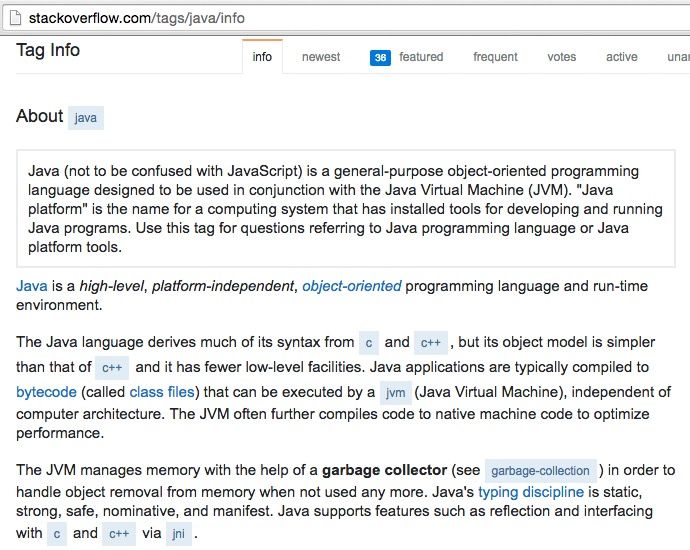
\includegraphics[width=5in]{chp6taginfo.jpg}  
\caption{The description for \textit{java} on StackOverflow dataset \footnote{\url{http://stackoverflow.com/tags/java/info} (accessed Feb 2016)}}
\label{fig:chp6taginfo} 
\end{figure}

Besides, each resource in DBpedia has a description.  We use DBpedia keyword lookup service \footnote{\url{http://dbpedia.org/projects/dbpedia-lookup}(accessed Feb 2016)} to retrieve related resource for each tag. As Shown in Figure \ref{fig:chp6lookup}, results of the lookup service are a lists of resources related to the given keyword.

\begin{figure}[htp]
\centering
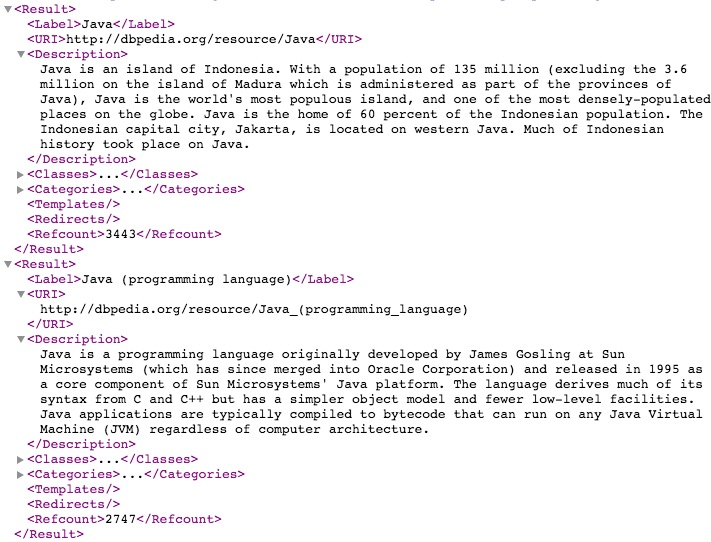
\includegraphics[width=5in]{chp6lookup.jpg}  
\caption{The example result of DBpedia lookup service for keyword \textit{java}}
\label{fig:chp6lookup} 
\end{figure}

In order to link \textit{java} to the correct DBpedia resource link. We compute the cosine similarity between the two descriptions from the two websites (StackOverflow and DBpedia) to solve the disambiguation problem. The  entire procedure is described as follows:

\begin{enumerate}
    \item{crawl the tag description from StackOverflow.}
    \item{retrieve DBpedia resources by the lookup service  }
    \item{compute the cosine distances between the description from StackOveflow and the description for each retrieved resource}
    \item{link the tag to the resource with the highest similarity}
\end{enumerate}


\subsection{Create graphs: retrieval potential links between resources}
After linking the tags to its corresponding DBpedia resources, we then perform several SPARQL queries to retrieve the potential relations among the resources found for each topic. 
\begin{itemize}
\item {Depth=1:} \\
select  ?relation \\
where\{ \\
\textit{ra} ?relation \textit{rb} . \\
\} 
\item{ Depth=2:} \\
select  ?r1, ?relation1, ?relation2 \\
where\{ \\
\textit{ra} ?relation1 ?r1 . \\
?r1 ?relation2 \textit{rb} .\\
\} 
\item{ Depth=3:} \\
select  ?r1, ?r2 ?relation1, ?relation2, ?relation3 \\
where\{ \\ 
 \textit{ra} ?relation1 ?r1 . \\
 ?r1 ?relation2 ?r2 .\\
 ?r2 ?relation3 \textit{rb} .\\
\} 
\end{itemize}
%TODO FAB: queries would be better presented as code.

Where, \textit{ra}, \textit{rb} are the resources for which we want to retrieve the potential relations. $?r1$, $?r2$, $?relation1$, $?relation2$, $?relation3$ are the potential relations and the intermediate resources. $Depth$ denotes the hops between the resources \textit{ra} and \textit{rb}. We vary this parameter by $1,2,3$. Figure \ref{fig:chp6resourcegraph} shown a retrieved graph for a linux related topic.
%TODO FAB: we have to explain why we don't use path expressions and what is the general idea behind these queries I propos the text below
To remain compatible with SPARQL 1.0 we did not use the path operator that would support a much synthetic way of writing these queries. The general idea behind these queries is to reconstruct a small connected graph around the detected resources for a topic in order to obtain a space where to analyze their relations.

\begin{figure}[htp]
\centering
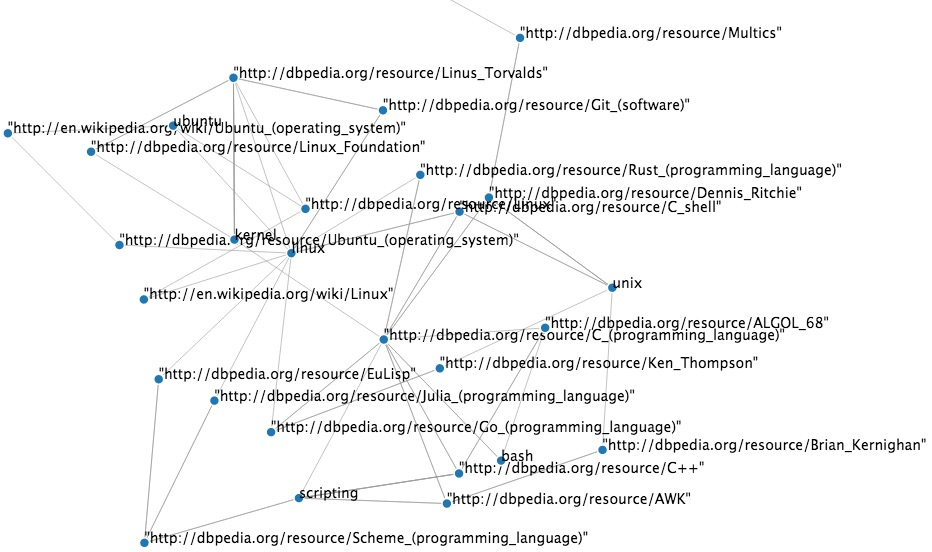
\includegraphics[width=5in]{chp6resourcegraph.jpg}  
\caption{The example graph structure for a linux topic}
\label{fig:chp6resourcegraph} 
\end{figure}

Once we have these relation graphs, we perform several graph algorithms to chose one or several resources as candidates to label the the bag of words of the topics. We mainly used the following algorithms/metrics:
\begin{itemize}
    \item {InDegree} \\
    In a directed graph, for a node, the number of head ends adjacent to a node is called the indegree of the node. 
    \item {Betweenness Centrality } \\
    It is an indicator of a node's centrality in a network. It is equal to the number of shortest paths from all vertices to all others that pass through that node.
    \item {Degree Centrality} \\
    It is defined as the number of links incident upon a node, which is equal to indegree plus outdegree for a directed graph.
    \item {Page Rank\cite{chp6page1999pagerank}}\\
    PageRank is an algorithm used by Google Search to rank websites in their search engine results. It can be applied on other kinds of graph to estimate the importance of the nodes.
    \item {Random} \\
    We just randomly choose one node from the graph.
    \item {Top tags} \\
    The topic modeling algorithm generates a topic-word distribution to indicate to what extent a word is related to a topic. By sorting words' corresponding probabilities, we can obtain a ranked word list for each topic, which are the top related words in each topic. A naive approach can use the first one or two tags to label each topic. 

\end{itemize}

\subsection{Experiments: A survey study}
In order to evaluate the performances of the different ways to generate labels we conducted user studies on the results. We designed two surveys for the user study. Table \ref{tab:chp6survey} shows the structure of the survey we used. For each survey, we listed 30 topics, half of them are from StackOverflow dataset, half of them are from Flickr dataset. The only difference for survey A and B is the linking (disambiguation) method. As mentioned in section \ref{sec:chp6secSolution}, we use both cosine similarity and babelfy to link tag with DBpedia resources. 

\begin{table}[htp]
\centering
\begin{tabular}{c|c|c}
\hline
             &  15 StackOverflow Topic& 15 Flickr Topic \\ \hline
    Survey A & Cosince Similairy & Babelfy\\ \hline  
    Survey B &  Babelfy          & Babelfy\\ \hline
\end{tabular}
\label{tab:chp6survey}
\end{table}


\subsubsection{Users' agreement}
We use Krippendorff’s Alpha\footnote{\url{https://en.wikipedia.org/wiki/Krippendorff's_alpha}} score to evaluate the degree of agreement among judges. The score indicates the homogeneity, or consensus, in the ratings given by judges. The score is always smaller than 1, $\alpha = 1 $ indicates the judges reach a perfect agreement and $\alpha =0 $ indicates the judges do not agree at all. When $\alpha <0 $ this means that judges reached a disagreement exceeding what can be expected by chance.  Figure \ref{fig:chp6alpha} illustrates the alpha score for 15 topics in each dataset and the average alpha score. We evaluate this score in three levels which correspond to the three sub figures. If we consider the top voted label as the best label, the first figure shows the agreement score among users. When we lower this limitation and consider the set of the top voted two labels as the best label, we can find that for most of the topics users could reach a good agreement. When we keep lowering this limitation and consider the top three voted labels as the best label, we can find there reach an excellent agreement. 



\begin{figure}[htp]
\centering
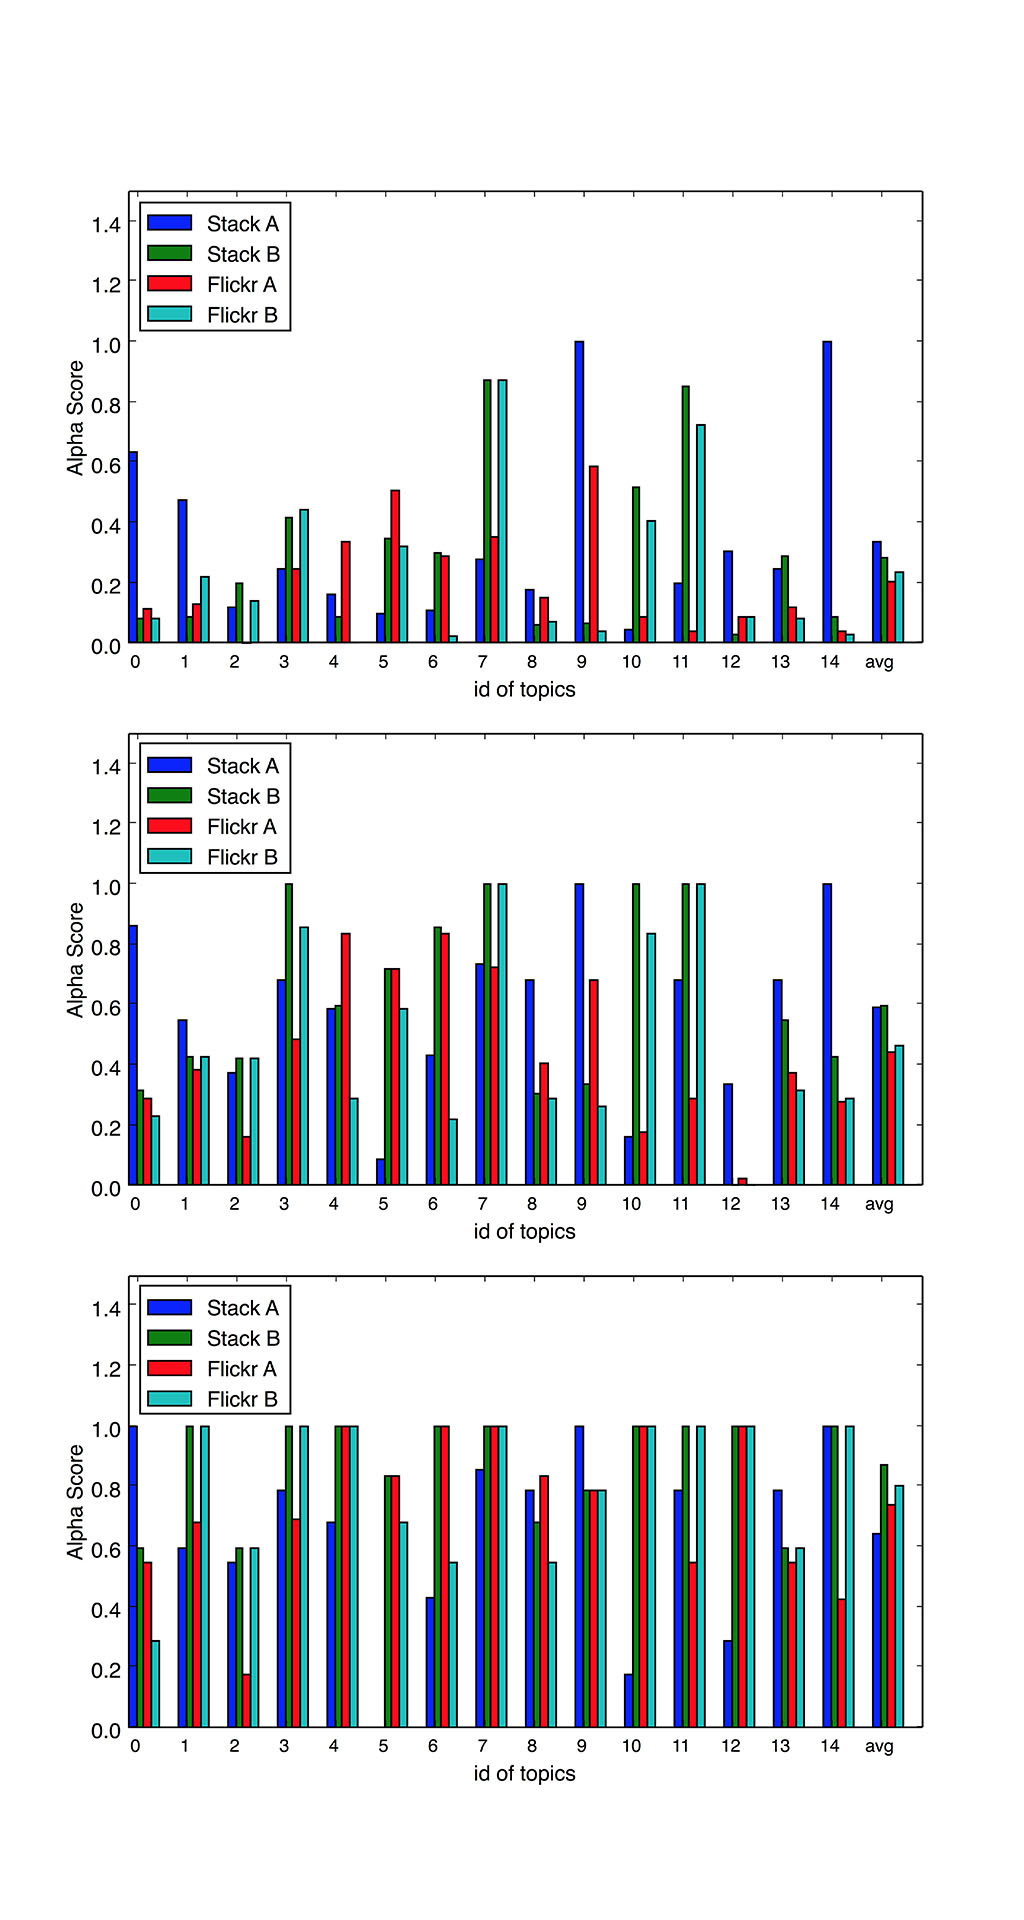
\includegraphics[width=5in]{chp6alpha.jpeg}  
\caption{}
\label{fig:chp6alpha} 
\end{figure}


In addition, we calculate the proportion of top voted labels. Figure \ref{fig:chp6top} shows the number of topics which top voted labels take a certain proportion. X-axis are the proportion, Y-axis are the number of topics. A data point ($50\%$,6) in the first sub figure means that there are 6 topics which first voted labels takes $50\%$ percent of all voted labels. A data point ($50\%$,6) in the second sub figure means that there are 6 topics which top two voted labels take $50\%$ percent of all voted labels. Similarly, A data point ($50\%$,6) in the third sub figure means that there are 6 topics which top three voted labels take $50\%$ percent of all voted labels. We can find that most of the labels chosen by judges are actually highly voted labels, which means all judges tend to agree on the top two or three labels.

\begin{figure}[htp]
\centering
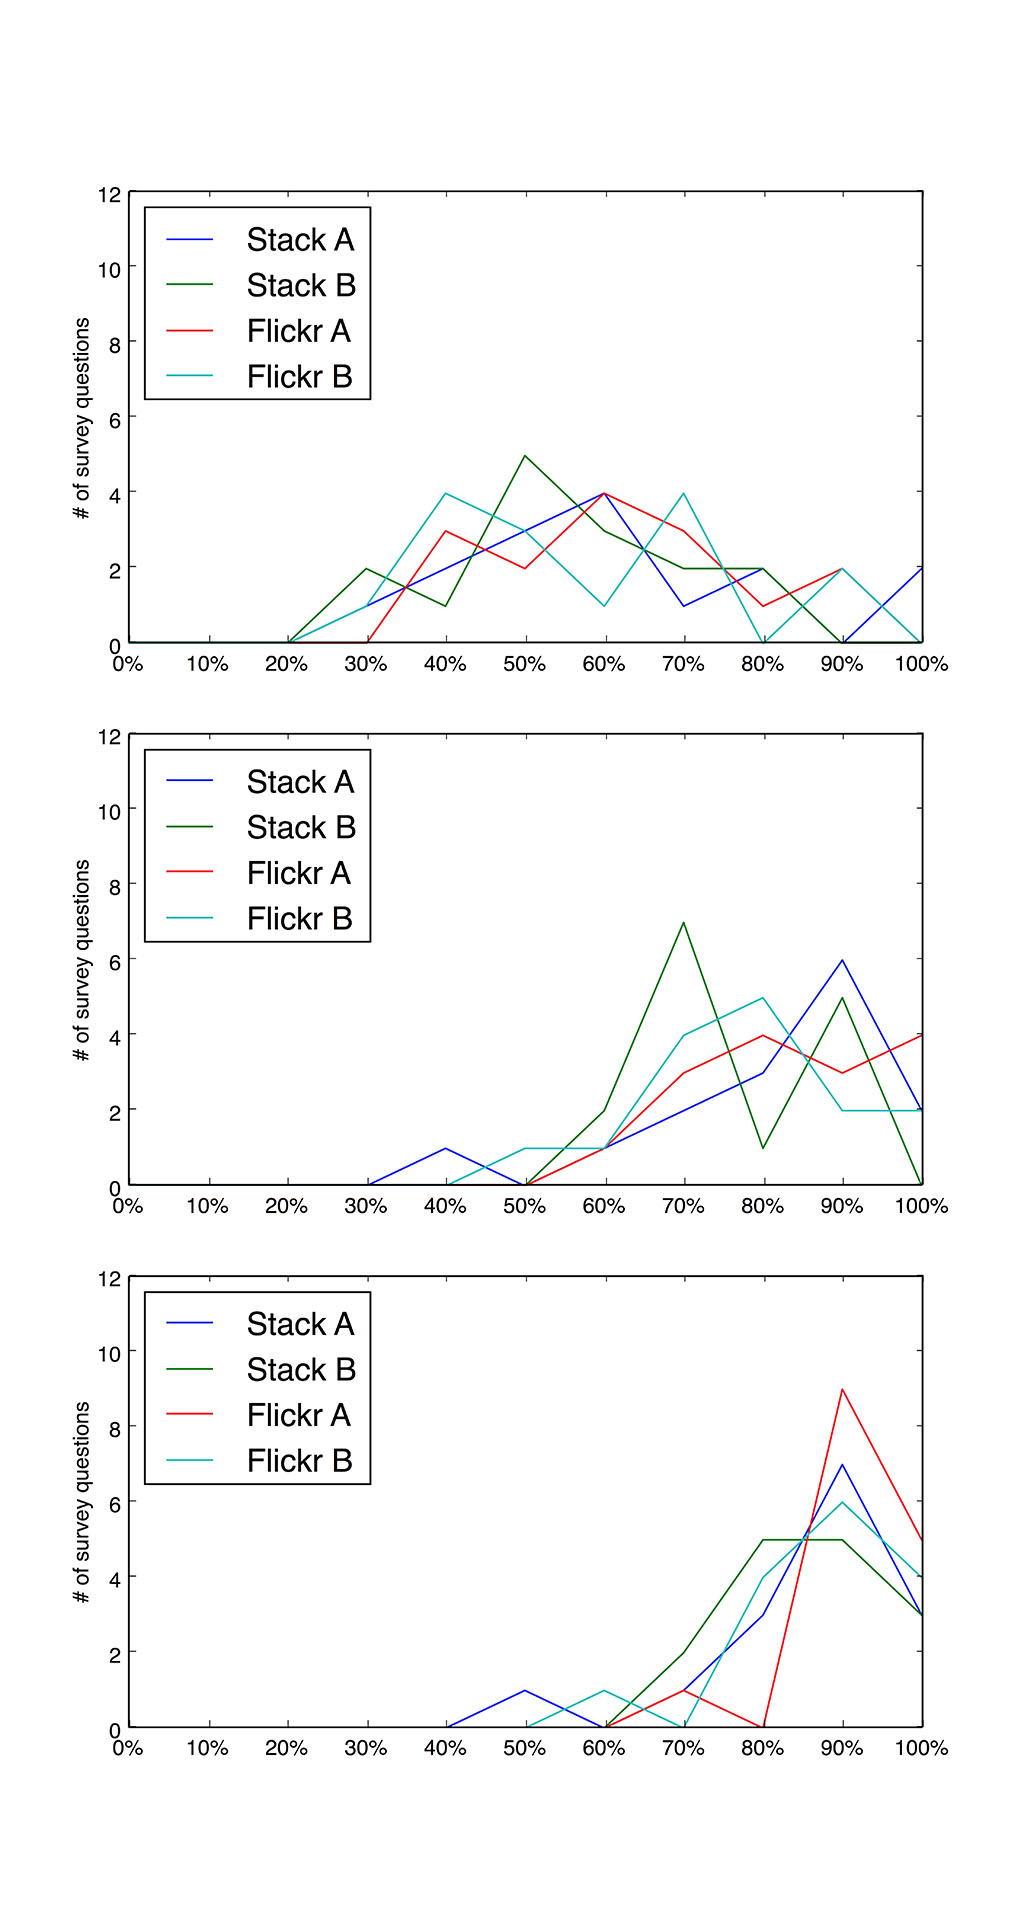
\includegraphics[width=5in]{chp6top.jpeg}  
\caption{}
\label{fig:chp6top} 
\end{figure}


\subsubsection{Quality evaluation: NDCG measurement}
We use NDCG metric to evaluate all the algorithms listed in Section \ref{sec:chp6secSolution}. The Normalized DCG (NDCG) is introduced to compare different ranking list. The value of NDCG is between 0.0 and 1.0. In our scenario, a NDCG@p value of 1.0 means detected interests and their order are totally the same as the labeled data until position \textit{p}, while a NDCG@p value of 0.0 means that the detected interests are completely different from the labeled data. For values between 0.0 to 1.0, it means that the detected interests are partially correct or ordered incorrectly. %It still 
Here, we evaluate NDCG@1, NDCG@2, and NDCG@3. The algorithm can generate a ranked label list. We sort the labels according to the number of votes from the survey as ideal ranking list. We also propose a method called \"Most+Top\". We created a label list by choosing a label which is the most recommended by all algorithms and labels from the \"Top tags\" algorithm. We can find that most of the algorithms can predict the good labels for a topic. Especially, if we consider giving two labels for a topic, our proposed method has very good results on all the datasets, which means for all the topics, the method can generate two good labels to represent the meaning of the topic.

\begin{figure}[htp]
\centering
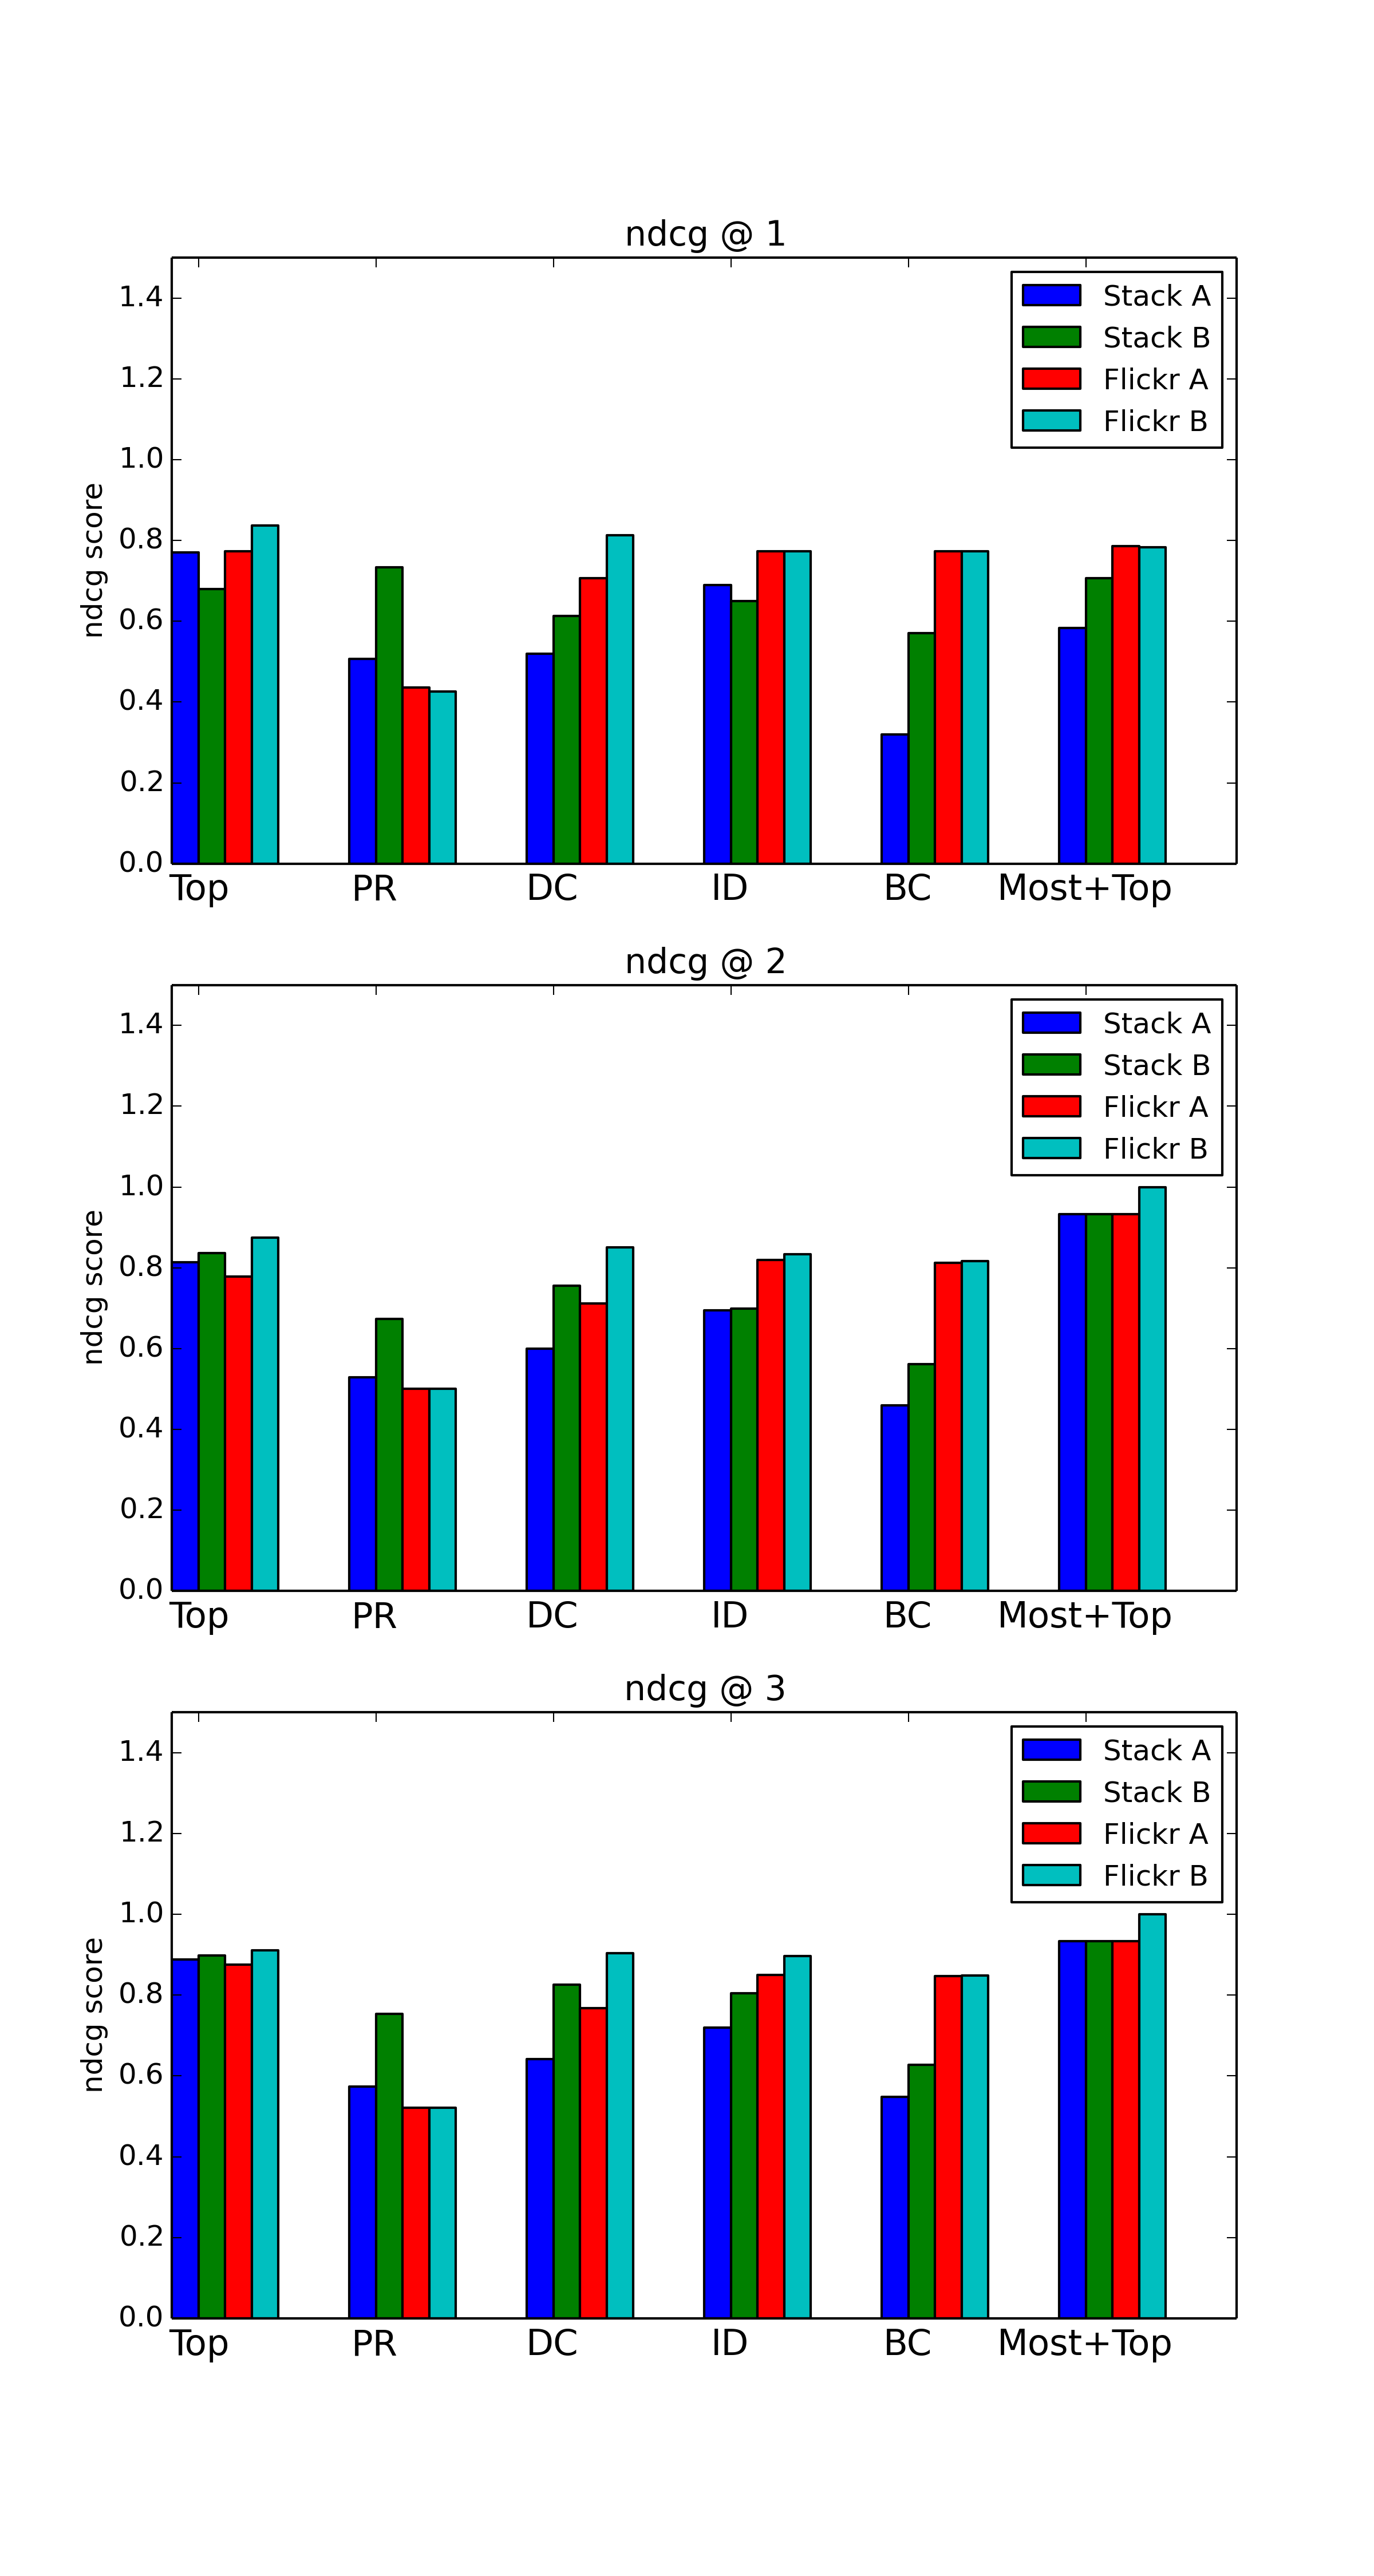
\includegraphics[width=5in]{chp6ndcg.jpeg}  
\caption{}
\label{fig:chp6ndcg} 
\end{figure}




\section{summary: represent a topic with labels}
In this chapter, we discussed how we used DBpedia as external knowledge to help choosing labels to turn bags of words into meaningful topics. From the user survey we found that users can reach a good agreement on a composite labels. Therefore, it is more reasonable to have more than one keyword to label the bag of words of atpoic. We also proposed a hybrid solution by combing results from different algorithms to generate composite labels to represent a topic. In the next chapter, we will focus on how to extract more sophisticated social information such as expertise, activity and trends.
